\section{Microeconomics Midterm 2018 / 19}

{
\subsection*{Schmidt}

{
\subsubsection*{Exercise 1}

\begin{enumerate}[label=(\alph*)]
{\item 
Violation of WARP:

$$
\left|\begin{array}{l}
p y^{\prime} \leqslant w \\
p^{\prime} y \leqslant w^{\prime}
\end{array}\right|
$$

Plug in the prices \& incomes (by Walras Law):

$$
\begin{aligned}
& \left|\begin{array}{rl}
30(12+x) & \leqslant 600 \\
540 & \leqslant 360+24 x
\end{array}\right| \\
& \Leftrightarrow\left|\begin{array}{c}
x \leq 8 \\
7.5 \leqslant x
\end{array}\right|
\end{aligned}
$$

Thus, WARP is violated if $x \in[7.5,8]$.
}
{\item 
For this, bundle from year 2 must be affordable in year 1:

$$
x \leq 8
$$

But we exclude all $x$ for which WARP is violated and find: $x \in[0,7.5)$
}
{\item 
The quantity has increased, so the income must have decreased to find $\frac{\partial y_{2}}{\partial w}<0$ :

$$
\begin{aligned}
600 & <360+24 x \\
\Leftrightarrow \quad 10 & <x
\end{aligned}
$$
}
\end{enumerate}
}
{
\subsubsection*{Exercise 2}

\begin{enumerate}[label=(\alph*)]
{\item 
Use hint because if $g(h(\cdot))$ represents preferences, then any strictly monotone transformation does it as well.
Thus $h(\cdot)$ represents the preferences \& is homogeneous. 
Call $h(\cdot)$ now $u(\cdot)$: 

EMP:

\begin{align*}
    \min _{x} p x \\
    \text{ s.t. } u(x)=1
\end{align*}

FOC:

\begin{align*}
    p_{l}-\lambda \frac{\partial u(x)}{\partial x_{l}}=0 \quad \forall l
\end{align*}

by Euler

$$
e(p, u=1)=\sum_{l} p_{l} x_{l}=\lambda \sum_{l} x_{l} \frac{\partial u(x)}{\partial x_{l}}=\lambda
$$

now let $u(x)=u$:

\begin{align*}
    \min _{x} p x \\
    \text{ s.t. } u(x)=u
\end{align*}

FOC:

$$
\begin{aligned}
    p_{l}-\lambda \frac{\partial u(x)}{\partial x_{l}}=0 \quad \forall l \\
    e(p, u)=\sum_{l} p_{l} x_{l} 
    =\lambda \sum_{l} x_{l} \frac{\partial u(x)}{\partial x_{l}} 
    =\lambda u=u \cdot e(p)
\end{aligned}
$$
}
{\item 
UMP:

$$
\begin{gathered}
    \max _{x} u(x) \\
    \text { st. } p x=1
\end{gathered}
$$

FOC:

$$
\begin{gathered}
\frac{\partial u(x)}{\partial x_{l}}-\lambda p_{l}=0 \quad \forall l \\
\Leftrightarrow \frac{\partial u(x)}{\partial x_{l}}=\lambda p_{l} \quad \mid \cdot x_{l} \\
\frac{\partial u(x)}{\partial x_{l}} x_{l}=\lambda p_l x_{l}
\end{gathered}
$$

Sum over $x_{l}$ and use Euler:

\begin{align*}
    \sum_{l} \frac{\partial u(x)}{\partial x_{l}} x_{l}=\lambda \sum_{l} p_l x_{l}  \tag{I} \\
    u\left(x^{*}\right)=v(p)=\lambda p x=\lambda
\end{align*}


Let $p x=1$ : Same $F O C$ and up to (I) nothing changes:

\begin{align*}
    & \sum_{l} \frac{\partial u(x)}{\partial x_{l}} x_{l}=\lambda \sum_l p_l x_{l} \\
    & u\left(x^{*}\right)=v(p, w)=\lambda p x=\lambda w=v(p) w \tag{II}
\end{align*}
}
{\item 
Follows from applying Roy's identity to (II):

$$
x_{l}(p, w)=-\frac{\frac{\partial v(p, w)}{\partial p_{l}}}{\frac{\left.\partial v p_{1} w\right)}{\partial w}}=-\frac{\frac{\partial v(p)}{\partial p_{l}} w}{v(p)}=x_{l}(p) w
$$
}
\end{enumerate}
}
{
\subsubsection*{Exercise 3}

\begin{enumerate}[label=(\alph*)]
{\item 
Leontief implies: $x_{1}^{*}=x_{2}^{*}$ and $u=x_{1}^{*}=x_{2}^{*}$ Thus, they must be able to afford the old bundle as Leontief does not allow for substitutions. They will also choose to consume it.

Before moving: $p_{1}=p_{2}=1$

$$
\rightarrow \quad x_{1}^{*}=x_{2}^{*}=\frac{w}{2}=500=u_{0}
$$

After moving: Set $u_{1}=u_{0}$. Thus

$$
x_{1}^{*}=x_{2}^{*}=500
$$

to afford this:

$$
e(p, u)=500(1+4)=2500
$$

As initial wage is 1000, we have $R=1500$.

This is the negative of CV.
}
{\item 
This is Cobb Douglas utility. Thus

$$
x_{1}^{*}=\frac{w}{2 p_{1}} \quad ; \quad x_{2}^{*}=\frac{w}{2 p_{2}}
$$

Before moving:

$$
\begin{aligned}
& x_{1}^{*}=x_{2}^{*}=500 \\
& v(p, w)=500
\end{aligned}
$$

After moving:

$$
v(p, w)=(w+R)\left(\frac{1}{2 p_{1}}\right)^{1 / 2}\left(\frac{1}{2 p_{2}}\right)^{1 / 2}=500
$$

$$
\Leftrightarrow \quad w+R=2000 \Leftrightarrow R=1000
$$

As CD utility allows for substitution, they choose to buy less of $x_{1}$ as it has become much more expensive.
}
\end{enumerate}
}
{
\subsubsection*{Exercise 4}

\begin{enumerate}[label=(\alph*)]
{\item 
This agent exhibits decreasing absolute risk aversion.

$$
r^{A}=-\frac{u^{\prime \prime}(x)}{u^{\prime}(x)}=-\frac{-\rho\left(1_{-\rho}\right)_{x}-\rho-1}{(1-\rho)_{x}^{-\rho}}=\rho x^{-1}
$$
}
{\item 
Agent maximizes expected utility:

$$
\max _{a} \int u(W-a W+a W \pi) d F(\pi)
$$

Assume interior solution:

$$
\text { FCC: } \quad \int u^{\prime}(w-a w+a W \pi)(\pi w-w) d F(\pi)=0
$$

Plug in functional form:

$$
\begin{aligned}
& \int(1-\rho)(1-a+a \pi)^{-\rho}(\pi-1) w^{1-\rho} d F(\pi)=0 \\
\Leftrightarrow & \underbrace{(1-\rho) w^{1-\rho}}_{\neq 0} \int(1-a+a \pi)^{-\rho}(\pi-1) d F(\pi)=0 \\
\Rightarrow \quad & \quad \int(1-a+a \pi)^{-\rho}(\pi-1) d F(\pi)=0
\end{aligned}
$$

This expression implicitly defines $a^{*}$ and is independent of $W$.
}
\end{enumerate}
}
}

{
\subsection*{Gottardi}

{
\subsubsection*{Exercise 1}

\begin{enumerate}[label=(\roman*)]
{\item 
\underline{Consumer A:}

$$
\begin{aligned}
& \max _{x_{1}^{A}, x_{2}^{A}} \ln \left(x_{1}^{A}\right)+2 \ln \left(x_{2}^{A}\right) \\
& \text { s.t. } p x_{1}^{A}+x_{2}^{A}=16 p
\end{aligned}
$$

FOC:

$$
\begin{aligned}
    & \left[x_{1}^{A}\right]: \frac{1}{x_{1}^{A}}-\lambda p=0 \\
    & {\left[x_{2}^{A}\right]: 2 \frac{1}{x_{2}^{A}}-\lambda=0} \\
    & \longrightarrow x_{2}^{A}=2 x_{1}^{A} p\longrightarrow x_{1}^{A}=\frac{16}{3}
\end{aligned}
$$

\underline{Consumer B:}

\begin{align*}
    \max _{x_{1}^{B} x_{2}^{B}} \ln \left(x_{1}^{B}\right)+\ln \left(x_{2}^{B}\right) \\
    \text{s.t. } p x_{1}^{B}+x_{2}^{B}=12
\end{align*}

FOC: 

\begin{align*}
    & \left[x_{1}^{B}\right]: \frac{1}{x_{1}^{B}}-\lambda p=0 \\
    & \left[x_{2}^{B}\right]: \frac{1}{x_{2}^{B}}-\lambda=0 \\
    & \longrightarrow x_{2}^{B}=x_{1}^{B} p \longrightarrow x_{2}^{B}=6
\end{align*}

\underline{Markets:}

$$
x_{1}^{A}+x_{1}^{B}=16 \quad ; \quad x_{2}^{A}+x_{2}^{B}=12
$$

$$
\Leftrightarrow x_{1}^{B}=16\frac{2}{3} \quad \Leftrightarrow \quad x_{2}^{A}=6
$$

Combine with either $F O C$ to find:

$$
\begin{aligned}
x_{2}^{B} &= p x_{1}^{B} \\
6 &= p 16\frac{2}{3} \\
p &= 9 / 16
\end{aligned}
$$

\underline{Competitive Equilibrium:}

$$
\begin{aligned}
\left(x_{1}^{A}, x_{2}^{A}\right) & =(16 \cdot \frac{1}{3},6) \\
\left(x_{1}^{B}, x_{2}^{B}\right) & =(16 \cdot \frac{2}{3},6) \\
p & =9 / 16
\end{aligned}
$$
}
{\item 
$$
M R S^{A}=\frac{x_{2}^{A}}{2 x_{1}^{A}} \stackrel{!}{=} M R S^{B}=\frac{x_{2}^{B}}{x_{1}^{B}}
$$

Use market clearing: $\quad x_{1}^{B}=16-x_{1}^{A}$

\begin{align*}
& \longrightarrow \quad \frac{x_{2}^{A}}{2 x_{1}^{A}}=\frac{12-x_{2}^{A}}{16-x_{1}^{A}} \\
& \Leftrightarrow \quad \frac{16-x_{1}^{A}}{2 x_{1}^{A}}=\frac{12}{x_{2}^{A}}-1 \\
& \Leftrightarrow \quad \frac{16-x_{1}^{A}+2 x_{1}^{A}}{2 x_{1}^{A}}=\frac{12}{x_{2}^{A}} \\
& \Leftrightarrow \quad x_{2}^{A}=\frac{24 x_{1}^{A}}{16+x_{1}^{A}} \tag{I}
\end{align*}

\begin{figure}[!htp]
    \centering
    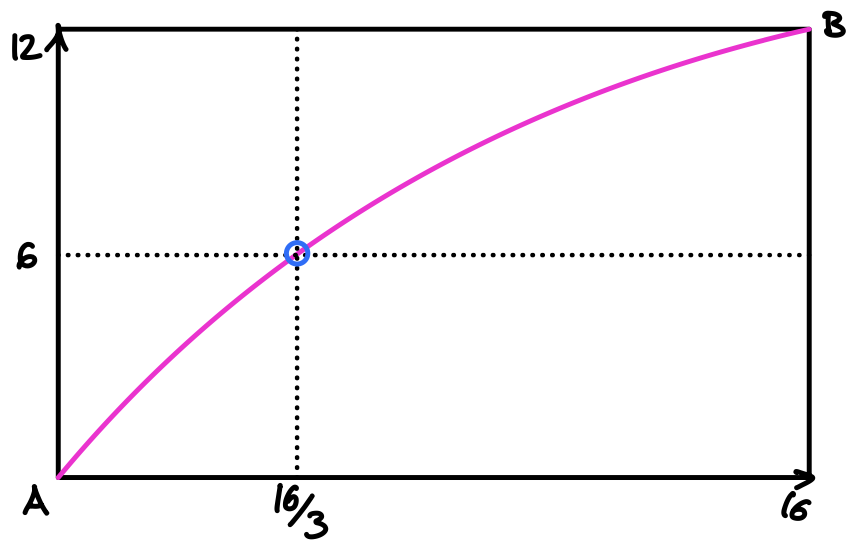
\includegraphics[width=.75\textwidth]{images/2018_19_1.png}
\end{figure}
}
{\item 
Plugging into $(I)$ :

$$
\begin{aligned}
& 8=\frac{24 \cdot 8}{16+8} \\
& 8=8
\end{aligned}
$$

Yes, it is PE.

Find transfers:

$$
\begin{aligned}
& T^{A}=\left[\begin{array}{l}
x_{1}^{A} \\
x_{2}^{A}
\end{array}\right]-\left[\begin{array}{l}
w_{1}^{A} \\
w_{2}^{A}
\end{array}\right]=\left[\begin{array}{l}
8 \\
8
\end{array}\right]-\left[\begin{array}{l}
16 \\
0
\end{array}\right]=\left[\begin{array}{c}
-8 \\
8
\end{array}\right] \\
& T^{B}=\left[\begin{array}{l}
x_{1}^{B} \\
x_{2}^{B}
\end{array}\right]-\left[\begin{array}{l}
w_{1}^{B} \\
w_{2}^{B}
\end{array}\right]=\left[\begin{array}{l}
8 \\
4
\end{array}\right]-\left[\begin{array}{c}
0 \\
12
\end{array}\right]=\left[\begin{array}{c}
8 \\
-8
\end{array}\right]
\end{aligned}
$$

Prices given by MRS:

$$
p=M R S^{A}=M R S^{B}=1 / 2
$$
}
\end{enumerate}
}
{
\subsubsection*{Exercise 2}
\begin{enumerate}[label=(\roman*)]
{\item 
at $t=0$ :

$$
q_{1} \theta_{1}+q_{2} \theta_{2}=0
$$

at $t=1$ and $s=1$ :

$$
x_{1}=2 \theta_{1}+\theta_{2}+4
$$

at $t=1$ and $s=2$ : 

$$
\quad x_{2}=\theta_{1}+2 \theta_{2}+8
$$
}
{\item 
consumer solves:

$$
\begin{aligned}
& \max _{\theta_{1}, \theta_{2}} \frac{1}{2}\left[\ln \left(2 \theta_{1}+\theta_{2}+4\right)+\ln \left(\theta_{1}+2 \theta_{2}+8\right)\right] \\
& \text { s.t. } q_{1} \theta_{1}+q_{2} \theta_{2}=0
\end{aligned}
$$

FOCs:

$$
\begin{aligned}
& \left[\theta_{1}\right]:\left(2 \theta_{1}+\theta_{2}+4\right)^{-1}+\frac{1}{2}\left(\theta_{1}+2 \theta_{2}+8\right)^{-1}-\lambda q_{1}=0 \\
& \left[\theta_{2}\right]: \frac{1}{2}\left(2 \theta_{1}+\theta_{2}+4\right)^{-1}+\left(\theta_{1}+2 \theta_{2}+8\right)^{-1}-\lambda q_{2}=0
\end{aligned}
$$

Suppose $q_{1}=q_{2}=1$ :

\begin{align*}
\frac{1}{2}\left(2 \theta_{1}+\theta_{2}+4\right)^{-1} & =\frac{1}{2}\left(\theta_{1}+2 \theta_{2}+8\right)^{-1} \\
2 \theta_{1}+\theta_{2}+4 & =\theta_{1}+2 \theta_{2}+8 \\
\theta_{1} & =\theta_{2}+4 \tag{II}
\end{align*}

Market clearing: $\theta_{1}=-\theta_{2}=0$ as there is only one consumer. This violates (II). Thus $q_{1}=q_{2}=1$ is not possible!

This result is the consequence of risk-aversion. The consumer is poorer in state 1, so she wants to buy insurance against it via asset 1. Unfortunately, she cannot because there is nobody else in the economy to trade with. To offset this excess demand for asset $1$ we must have $q_{1}>q_{2}$ which makes it less attractive.
}
{\item 
There is no risk aversion and therefore the assets are not interesting as an insurance as they have the same expected return. As a consequence the prices reflect the state probabilities. As $\pi_{1}=\pi_{2}=1 / 2$, will find $q_{1}=q_{2}$ and $q_{1}=q_{2}=1$ is a CE.
}
\end{enumerate}
}
}